\appendix
\chapter{Presupuesto y Planificación}
\section{Presupuesto}

El presupuesto del trabajo se puede separar en tres partes: recursos humanos, compra de material y amortización de los equipos utilizados.

En cuanto a los recursos humanos empleados, se ha tenido una dedicación por parte del alumno de unas 800 horas, esto es un número de horas mucho superior a las 360 horas (30h/ECTS) correspondientes a la carga temporal de los 12 ECTS del Trabajo fin de Grado (TFG). Esto se ha debido al gran alcance y a la complejidad del mismo. Un sueldo de investigador a media jornada en la universidad, sin estar graduado, es de unos 450 euros. Lo que se traduce en un salario de unos 5,625 euros la hora. Los salarios del tutor y el cotutor se han extraído del portal de transparencia de la UPM. La dedicación del tutor ha sido de unas 20 horas de implicación en el trabajo y la implicación del cotutor ha sido de unas 80 horas de implicación.  

\begin{figure}[htb!]
		\centering
		\begin{tabular}{|l|r|r|r|}
		\hline
		%\textbf{Recursos humanos} &Coste unitario [EUR] &Unidades&Total [EUR]\\
		
		\textbf{Recursos humanos} & Horas &Coste Horario [EUR]&Total [EUR]\\
		\hline
		
		Alumno & 800 & 5.625 &  4500 \\
		Cotutor & 80 & 7.8 & 624\\
		Tutor & 20& 33.72 & 674.4 \\
		\hline
		\textbf{Total} & &  & \textbf{5798.4}\\
		\hline
		\end{tabular}\\
	
\end{figure}

Los costes de material del proyecto son debidos a la construcción del cuadricóptero y del autopiloto.


\begin{figure}[htb!]
	\centering
	\begin{tabular}{|l|r|r|r|}
		\hline
		\textbf{Material} &Coste unitario [EUR] &Unidades&Total [EUR]\\
		
		\hline
		
		\textbf{Cuadrirrotor}& & &  \\
		Bobina PLA 1Kg & 20 & 1.5 &  30 \\
		Perfiles aluminio & 2 & 1 & 2\\
		Pack 4 Motores MT2204 II & 25 &1& 25 \\
		ESC BlHeli 4 in 1  & 50 & 1 & 50\\
		Baterías LiPo & 25 & 2 & 50\\
		PCB autopiloto & 20 & 1 & 20\\
		Componentes PCB & 50 & 1  & 50 \\
		Hélices HQ5040 &2.5&4&10\\
		\hline
		\textbf{Total} & &  & \textbf{239}\\
		\hline
	\end{tabular}\\
\end{figure}

En cuanto a la amortización del equipo, se han empleado 2 ordenadores para el desarrollo del software y para el entrenamiento de los algoritmos. Se ha considerado una amortización lineal del 10 \% de la vida útil (10 años).

\begin{figure}[htb!]
	\centering
	\begin{tabular}{|l|r|r|r|}
		\hline
		\textbf{Equipo} & Precio &Coste Amortización(10\%)\\
		\hline
		
		Pc sobremesa & 1980 & 198\\
		Pc portátil & 1300 & 130\\
		\hline
		\textbf{Total} & & \textbf{328}\\
		\hline
\end{tabular}\\
\end{figure}

Añadiendo un coste de encuadernado de la memoria de unos 30 euros el presupuesto total del proyecto ha sido



\begin{figure}[htb!]
	\centering
	\begin{tabular}{|l|r|r|r|}
		\hline
		\textbf{Concepto} &Total [EUR]\\
		\hline
		Recursos humanos & 5798.4\\
		Material &239\\
		Amortización del equipo & 328\\
		Encuadernación&40\\
		
		\hline
		\textbf{Total}   & \textbf{6405,4}\\
		\hline
	\end{tabular}\\
\end{figure}





\section{Planificación}
La realización de este trabajo ha empleado un ritmo continuo de horas de trabajo desde su comienzo, siendo un poco menor en épocas de exámenes y un poco mayor al comienzo de los cuatrimestres y julio. La dedicación media diaria del trabajo ha sido de unas 4 horas semanales, durante un periodo de unos 10 meses (descontando agosto y septiembre), lo que da un total de unas 800 horas. La inmensa mayoría de estas horas se han dedicado en el Centro de Automática y Róbotica (CAR) de la Escuela Técnica Superior de Ingenieros Industriales (ETSII) de la Universidad Politécnica de Madrid (UPM), concretamente en el grupo de investigación de Visión por Computador y Robots Aereos (CVAR).

En cuanto a la distribución del trabajo en este tiempo, el trabajo comenzó a realizarse en septiembre de 2018, durante los primeros meses se realizó el curso sobre redes neuronales y aprendizaje profundo, en la plataforma online Coursera. La duración del curso se extendió hasta finales de diciembre. Paralelamente, a partir de octubre se comenzó con el diseño de la aeronave, y en noviembre con el del autopiloto. A principios de febreró se finalizo con el diseño y construcción del cuadricóptero y con el diseño y montaje de la PCB del autopiloto. A partir de este punto, el resto del tiempo se ha dedicado al software, tanto el del autopiloto, como el de la estación de tierra , al diseño de los algoritmos de control y a la experimentación real. Se ha realizado un diagrama GANTT (\cref{gantt}) en el que se ha detallado más en profundidad la distribución temporal de las tareas. Asimismo, se ha esquematizado la organización del proyecto en un diagrama EDP (\cref{EDP}). 

\begin{figure}[htb!]
	\centering
	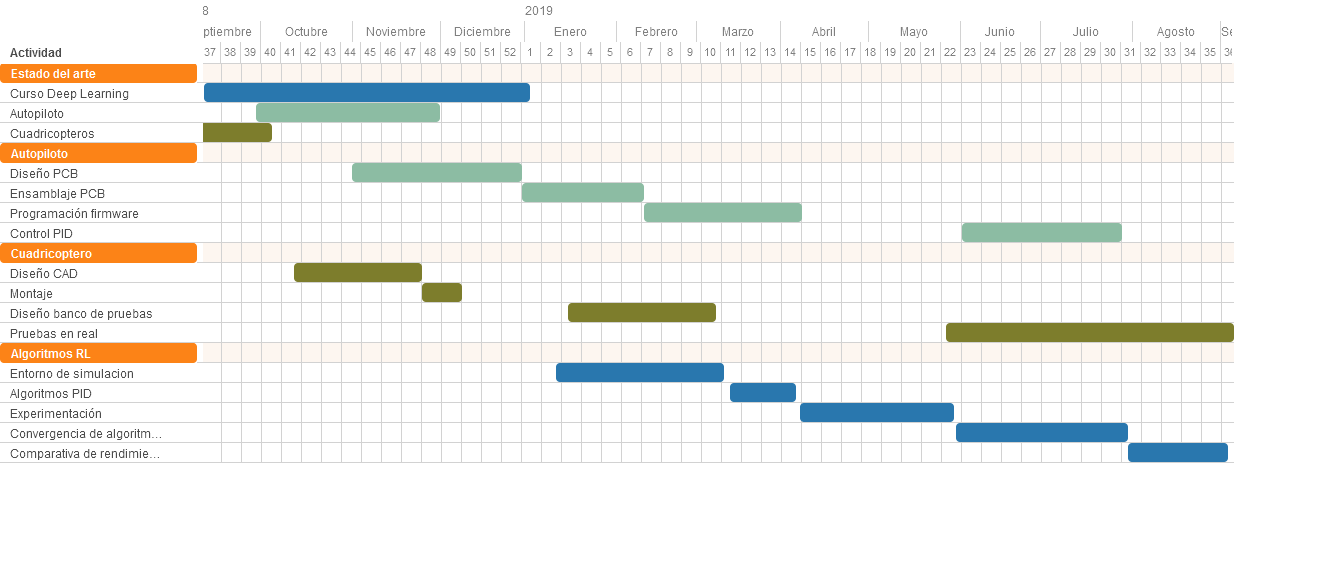
\includegraphics[width=\textwidth]{planificacion_ambiental/gantt}
	\caption{Diagrama de Gantt}
	\label{gantt}	
\end{figure}

\begin{figure}[htb!]
	\centering
	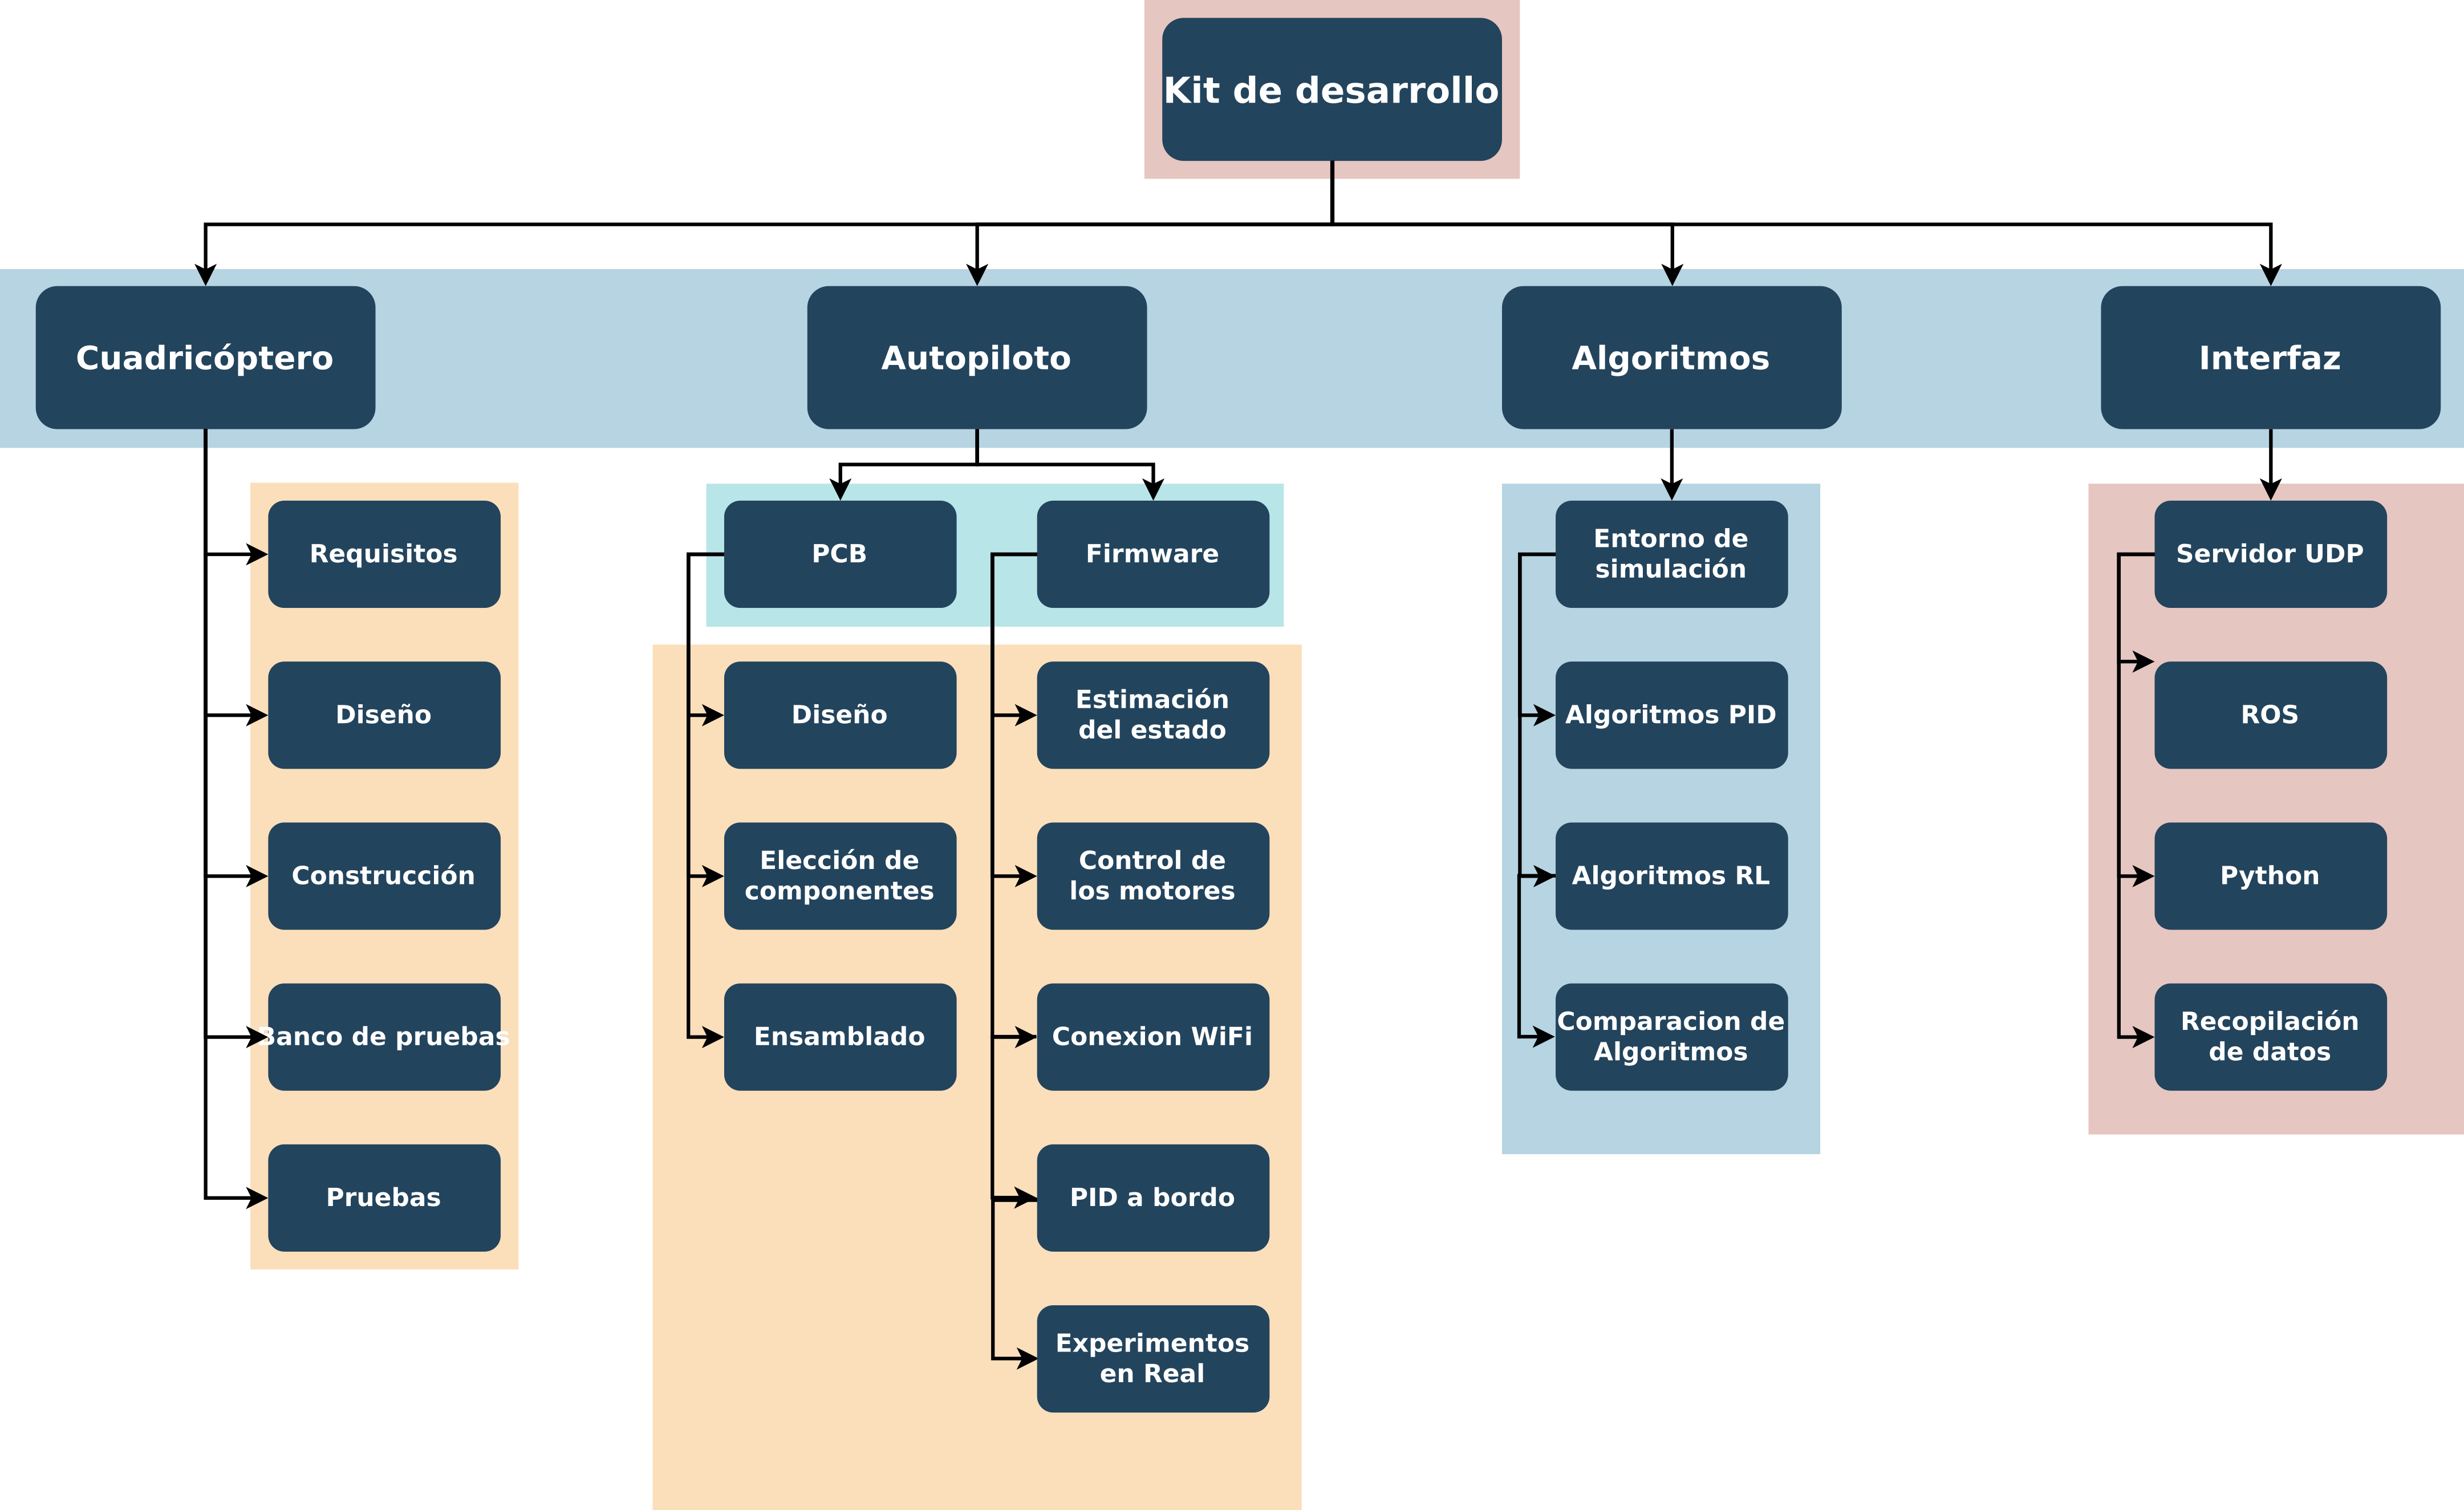
\includegraphics[width=\textwidth]{planificacion_ambiental/edp}
	\caption{Diagrama EDP}
	\label{EDP}	
\end{figure}



\chapter{Impacto social y medioambiental}

El impacto social que tiene este trabajo se ve reflejado en su posible empleo en la educación y la investigación. Actualmente las metodologías docentes están tendiendo hacia el aprendizaje práctico, hacia aprender haciendo. Esta plataforma podría emplearse en centros docentes debido a su montaje mecánico hecho casi en su totalidad con impresion 3D.

Desde el punto de vista de la investigación, tener la posibilidad de desarrollar y probar nuevos algoritmos para el control de drones puede mejorar la efectividad del uso de estas aeronaves en múltiples aplicaciones. Cuanto mejor sea el controlador, más fácil será utilizar estas aeronaves para tareas de inspección, seguridad y busqueda y rescate, entre otras.

El impacto medioambiental de la plataforma es reducido, ya que, el PLA es un plástico biodegradable y las baterías de Litio, una vez descargadas, son sencillas de desechar. EL proceso de fabricación de los componentes requiere de recursos materiales y energéticos, cuyo proceso de obtención  puede povenir de fuentes no renovables. Sin embargo, los beneficios sociales que se pueden extraer de los resultados del proyecto hacen asumible este impacto medioambiental.


